\unnumberedChapter{Cab Handheld Hardware}

As described in the previous chapter, a cab handheld consists of a controller and a set of buttons, switches, and dials. It connects directly to the LCS bus and provides the controls needed to select a locomotive, set its speed and direction, and operate its functions.

This chapter describes the hardware implementation, starting with a development platform for the cab handheld firmware. Although this first version is not intended to be a compact handheld device, it contains essentially all the hardware elements needed for the final design.

\unnumberedSection{Cab Handheld Firmware Development Platform}

Typically, the first steps in firmware development are taken using a breadboard implementation of the hardware. But why not create a PCB with all the user interface elements right from the beginning?
Experience with breadboards has taught me that a dedicated PCB is considerably more robust. You will spend less time chasing firmware bugs that eventually turn out to be nothing more than a loose connection on a breadboard. This is, by the way, a lesson learned the hard way!

With the very reasonable prices of PCB manufacturing today, it is often easier to create a PCB quite early in the design phase. If something turns out to be wrong, simply correct the design and order another set of boards. Of course, one could also build the module on a general-purpose prototyping board. However, once the schematics are available, going one step further and creating a dedicated PCB is not much additional effort.
I find this a worthwhile investment, particularly when building a robust prototype that will be used throughout firmware development.

The following schematic shows the extension board developed for the cab handheld firmware. First, let’s look at the block diagram.

\unnumberedSubSection{Main Controller}

The main controller section essentially consists of a Raspberry Pi Pico, a CAN bus interface, and non-volatile memory. These components should be quite familiar by now.

Apart from the two I2C connections and the CAN bus signals, almost all GPIO pins are assigned to buttons or rotary encoders. Since the GPIO pins can be configured with internal pull-up resistors, no additional external pull-up resistors are required.

The board is powered from the LCS bus. Alternatively, it can also be powered directly through the Pico’s USB connection. This is particularly convenient during initial firmware development and debugging, as the handheld can be operated without connecting it to the layout.

The LCS bus connector provides the connection to the layout. For this application, we only need the CAN bus signals and, optionally, the power supply from the bus.

\begin{figure}[htbp]
\centering
\includegraphics[page=2, width=0.9\textwidth]{./part-cab-handheld/chapter-cab-handheld-hardware/Schematic_LcsNodes-Cab-Dev.pdf}
\caption{Main Controller}
\end{figure}
\FloatBarrier

\unnumberedSubSection{Interface}

The remaining part of the schematic contains the user interface elements: the buttons, rotary encoders, and OLED display. Together, these provide all the controls required for operating a locomotive and navigating the handheld’s configuration menus.
The following schematic completes the circuit design of the cab handheld development platform.

\begin{figure}[htbp]
\centering
\includegraphics[page=3, width=0.9\textwidth]{./part-cab-handheld/chapter-cab-handheld-hardware/Schematic_LcsNodes-Cab-Dev.pdf}
\caption{User Interface Elements}
\end{figure}
\FloatBarrier

Granted, this is not exactly a cab handheld that you would want to hold in your hands! Although the final version will use essentially the same hardware components, its form factor will naturally be quite different.

For firmware development, however, this setup is very convenient. All the necessary controls are readily accessible, and the dedicated PCB provides a robust platform for testing and debugging. Most importantly, you can concentrate on the firmware rather than chasing intermittent connections on a breadboard.

\unnumberedSubSection{PCB}

The following figure shows the PCB layout of the development platform. It is a 10cm by 12cm board with the UI elements placed like they would be placed on a true handheld. The PCB already gives us a hint how a cab handheld for holding in your hand could be arranged. 

\begin{figure}[htbp]
\centering
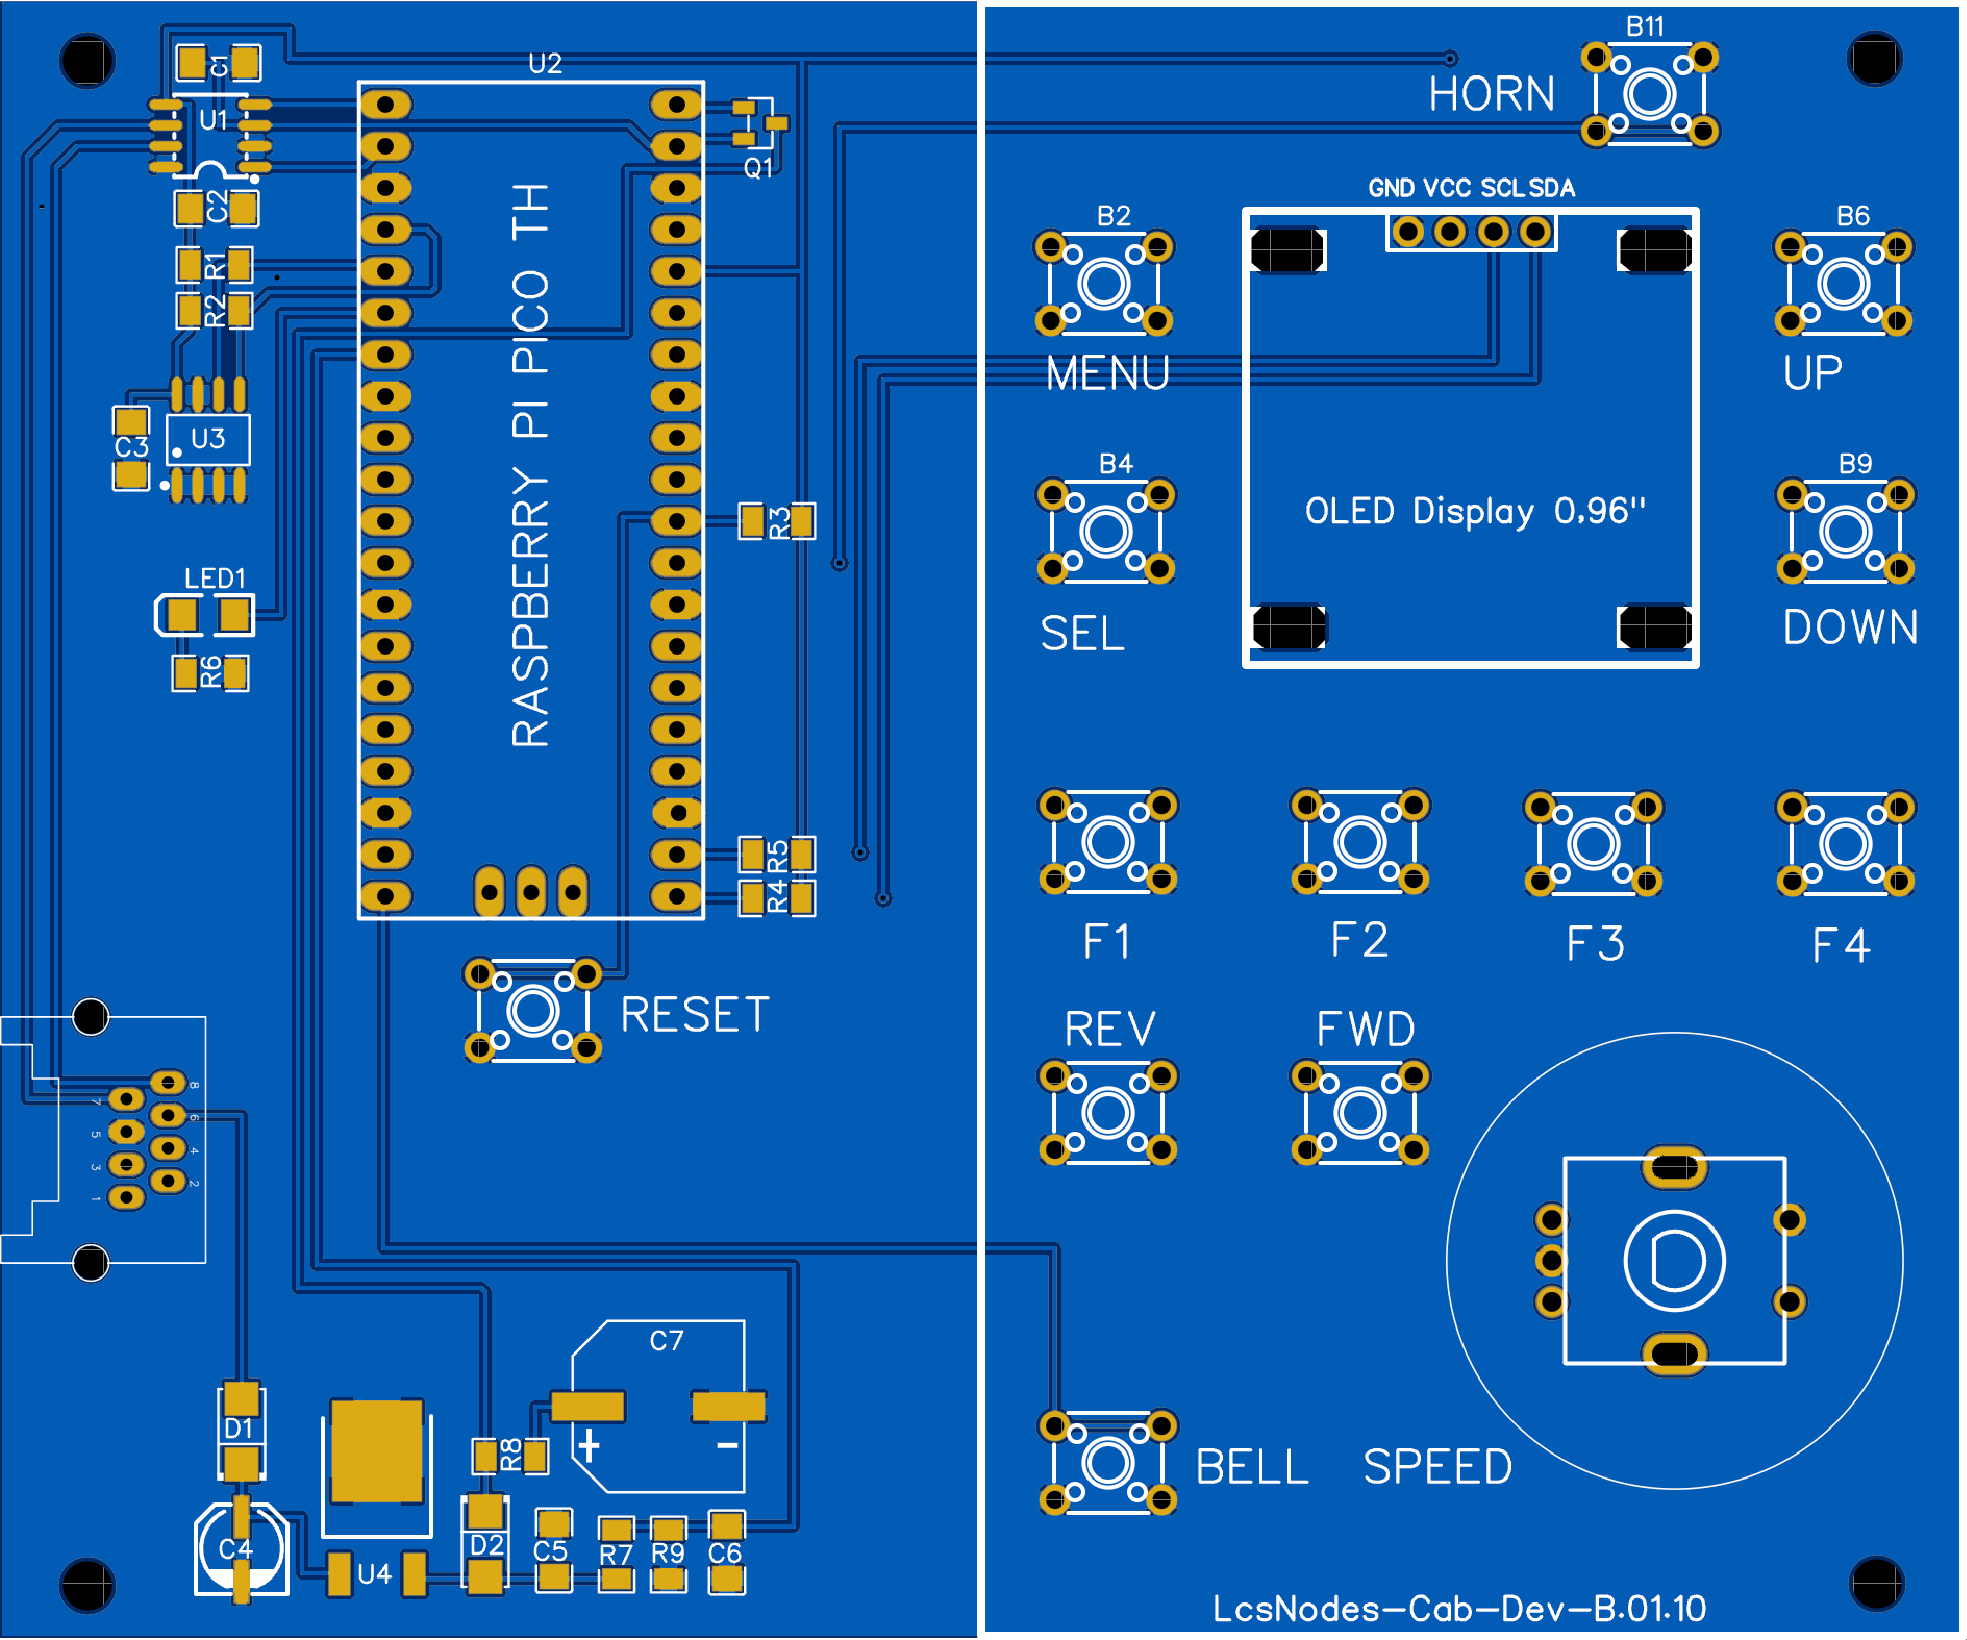
\includegraphics[width=0.9\textwidth]{./part-cab-handheld/chapter-cab-handheld-hardware/PCB_LcsNodes-Cab-Dev.pdf}
\caption{Cab Handheld Development Platform PCB}
\end{figure}
\FloatBarrier

The next subsection will dive into building our basic cab handheld. The design uses the same components, but will arrange them differently.

\unnumberedSection{A Basic Cab Handheld}

The basic cab handheld uses essentially the same hardware as the development platform described in the previous section. The main difference is the form factor. Instead of a development board with all components spread out for easy access, the components are arranged in a more compact layout suitable for actual operation.


??? TODO: Add block diagram and describe the final hardware implementation.

\begin{figure}[htbp]
\centering
% \includegraphics[page=2, width=0.9\textwidth]{./part-cab-handheld/chapter-cab-handheld-hardware/Schematic_LcsNodes-Cab-Dev.pdf}
\caption{Basic Cab Handheld}
\end{figure}
\FloatBarrier


\vspace{8em}

Phew! With the cab handheld, we have taken another big step towards actually operating a layout. After all, a layout control system without some form of cab handheld would be of rather limited use.

As mentioned before, there are many ways to build a cab handheld. The design of the user interface elements and their firmware was greatly influenced by a commercial handheld called \textbf{\textit{ProtoThrottle}}. In particular, the concept of navigating the display using four dedicated buttons surrounding the screen found its way into our UI Elements library.

Beyond a general-purpose cab handheld, it is also interesting to consider devices tailored to a particular class of locomotives. Such a handheld can reproduce the controls and operating experience of the actual locomotive.
The next section presents one such example: a diesel cab handheld inspired by the control stand of a diesel locomotive from the 1950s.


\unnumberedSection{The Diesel Cab Handheld}

The general-purpose cab handheld described earlier is just one possible approach to controlling a locomotive. A rather different concept is demonstrated by Iowa Scale Engineering with their \textbf{\textit{ProtoThrottle}}. This wireless handheld reproduces the control stand of a vintage diesel locomotive. And what a difference it makes!

Instead of setting the locomotive speed directly, the operator is provided with separate levers for the diesel engine’s prime mover, the direction, and the brakes.
Operating the locomotive becomes a much more realistic experience. First, the operator sets the prime mover to the desired notch and releases the brakes. The locomotive then starts moving. When the prime mover is returned to idle, the locomotive does not simply stop; it continues to roll until the brakes are applied.
In short, this provides a much more realistic way of operating a diesel locomotive than simply turning a speed knob.

Our diesel cab handheld adopts many of the design elements of the general-purpose cab handheld. It has a display surrounded by the same four navigation buttons: \texttt{MENU}, \texttt{SEL}, \texttt{UP}, and \texttt{DOWN}. The software configuration menus follow the same principles, so much of the firmware can be reused.
The four general-purpose function buttons, together with the dedicated horn and bell buttons, are also retained.

The main difference is in the locomotive controls. There is no longer a speed knob. Instead, the handheld provides separate throttle and brake levers. Direction is also controlled by a lever rather than the two dedicated direction buttons.

The following figure shows a rough sketch of the diesel cab handheld.

\begin{center}
    \begin{tikzpicture}[scale=0.9, transform shape]
        
     	\draw[help lines, gray!50, dashed] (0,0) grid(9,14);
     	
     	\node[ tsRoundedRectangle, 
                minimum width=9cm,
                minimum height=14cm,
                text width=3cm,
                text centered,
                fill=white!50] (display) at (4.5,7) { };

       	\node[ tsRoundedRectangle, 
                minimum width=3.5cm,
                minimum height=3.5cm,
                text width=3cm,
                text centered,
                fill=gray!30] (display) at (4.5,9.5) {Display};
        
        \node[ tsRoundedRectangle, 
                minimum width=2cm,
                minimum height=1cm,
                text width=2cm,
                text centered,
                fill=red!50] (horn) at (7,12.5) {Horn};
        
        \node[ tsRoundedRectangle, 
                minimum width=1cm,
                minimum height=1cm,
                text width=1cm,
                text centered,
                fill=blue!20] (menu) at (1.5,10.5) {Men};
                
      	\node[ tsRoundedRectangle, 
                minimum width=1cm,
                minimum height=1cm,
                text width=1cm,
                text centered,
                fill=blue!20] (up) at (7.5,10.5) {Up};

     	\node[ tsRoundedRectangle, 
                minimum width=1cm,
                minimum height=1cm,
                text width=1cm,
                text centered,
                fill=blue!20] (sel) at (1.5,8.5) {Sel};
                
    	\node[ tsRoundedRectangle, 
                minimum width=1cm,
                minimum height=1cm,
                text width=1cm,
                text centered,
                fill=blue!20] (down) at (7.5,8.5) {Dn};
                
     	\node[ tsRoundedRectangle, 
                minimum width=1cm,
                minimum height=1cm,
                text width=1cm,
                text centered,
                fill=red!50] (f1) at (1.5,6) {F1};
                
      	\node[ tsRoundedRectangle, 
                minimum width=1cm,
                minimum height=1cm,
                text width=1cm,
                text centered,
                fill=red!50] (f2) at (3.5,6) {F2};
                
      	\node[ tsRoundedRectangle, 
                minimum width=1cm,
                minimum height=1cm,
                text width=1cm,
                text centered,
                fill=red!50] (f3) at (5.5,6) {F3};
                
     	\node[ tsRoundedRectangle, 
                minimum width=1cm,
                minimum height=1cm,
                text width=1cm,
                text centered,
                fill=red!50] (f4) at (7.5,6) {F4};
                
      	\node[ tsRoundedRectangle, 
                minimum width=6cm,
                minimum height=0.75cm,
                text width=2cm,
                text centered,
                fill=green!50] (throttle) at (5,4.5) {Throttle};
                
                
       	\node[ tsRoundedRectangle, 
                minimum width=2cm,
                minimum height=0.75cm,
                text width=1cm,
                text centered,
                fill=green!50] (dir) at (6,3) {Dir};
                
      	\node[ tsRoundedRectangle, 
                minimum width=3cm,
                minimum height=0.75cm,
                text width=2cm,
                text centered,
                fill=green!50] (brake) at (2.5,2.5) {Brake};
                
       	\node[ tsRoundedRectangle, 
                minimum width=1cm,
                minimum height=1cm,
                text width=1cm,
                text centered,
                fill=red!50] (Bell) at (1.5,1) {Bell};
                
    \end{tikzpicture}
\end{center}

The main difference between the two handhelds is not just the arrangement of the controls but also the way a locomotive is operated. The general-purpose cab handheld sets the desired speed directly. The diesel cab handheld, on the other hand, provides separate controls for the prime mover, direction, and brakes. The locomotive’s actual speed is the result of these settings and the decoder’s response to them. This makes operating a diesel locomotive a considerably more realistic experience.

From a hardware perspective, the diesel cab handheld builds upon the design of the general-purpose handheld described in the previous section. The controller, display, navigation buttons, and function keys remain essentially unchanged. The only significant difference is the replacement of the speed knob with three dedicated levers for throttle, direction, and brakes.

This means that we can reuse much of the existing hardware design and, more importantly, much of the firmware infrastructure.
Let’s get started!

\unnumberedSubSection{Diesel Cab Handheld Requirements}

??? Very similar to the previous cab handheld, instead of speed knob, it features throttle and brake, all else is about the same...

\unnumberedSubSection{Diesel Cab Handheld Module hardware}

??? leverage the basic hardware, add analog inputs for throttle, break...

\unnumberedSubSection{Diesel Cab Handheld Module firmware}

??? UI elements are key again, leverage many screen built before, new part is how throttle and brake interplay to run the engine

\unnumberedSection{Summary}

We now have two different cab handhelds: a general-purpose handheld for controlling locomotives and a specialized diesel cab handheld that reproduces the controls of a diesel locomotive. Both share much of the same hardware and firmware infrastructure.

There is certainly room for further variations. One could imagine dedicated handhelds for steam or electric locomotives, each reproducing the characteristic controls of that particular type of engine. The existing firmware already provides much of the infrastructure needed to implement such variations without having to start from scratch.

And why stop at handhelds? Perhaps one day we will build a control panel that can be integrated into a fixed layout control desk, or Stellwerk. Such a design might use little more than a main controller and an extension board containing the appropriate UI Elements. The same hardware and software concepts could be used in quite different physical arrangements.

What about handhelds that also provide controls for other layout functions? Who knows. For now, I prefer to leave accessory control, such as operating turnouts, to dedicated layout control panels and computer-based control software. The handhelds described here deliberately focus on operating locomotives. They favor the idea of reproducing a locomotive control stand rather than providing yet another TV remote-style controller.

There are, of course, many other possibilities. The current design connects to the LCS bus via cable, but a wireless version would not be particularly difficult to implement. More or fewer buttons, a numeric keypad, or a completely different arrangement of controls are all perfectly valid alternatives. Ultimately, it is a matter of personal preference. So, feel free to build your own!

Finally, there is the question of connecting commercially available handhelds. This would require a gateway translating between their native protocols, such as LocoNet, and the LCS protocol. Connecting commercial handhelds through LCS gateways or base station interfaces is certainly a possibility for the future. For now, however, it remains on the backlog.